\section{Tickets}
\label{sec:tickets}

The HOPR protocol makes use of a custom micropayment scheme to process its incentives. This section focuses on the utilized micro-payment scheme and serves as a building block for section \ref{sec:incentives}.

Incentives are handled by a structure called \textit{tickets} that is inspired by payment channels as well as probabilistic payments and allows nodes to issue asset transfers without requiring each time an on-chain interaction. Tickets are sent locked and get unlocked afterwards, i. e. after proving that a packet has been relayed. Nodes who receive a locked ticket are able to validate its validity. Once a node has received the required cryptographic material to unlock the ticket, it is able to claim the incentive by submitting the ticket to the smart contract.

\begin{figure}[H]
    \centering
    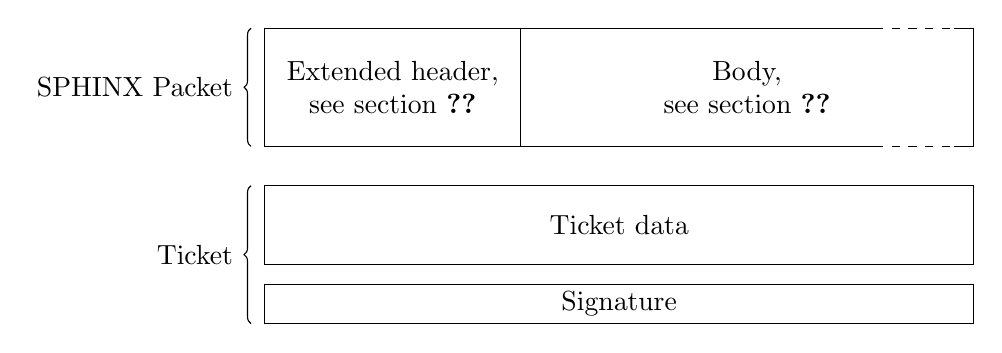
\begin{tikzpicture}[every text node part/.style={align=center}]
        \def\width{9}
        \def\headerWidth{9}
        \def\headerHeight{1.5}
        \def\headerOffset{3.25}
        \def\dashOffset{4.5}
        \def\dashWidth{1}

        \def\ticketDataHeight{1}
        \def\ticketSignatureHeight{0.5}

        \draw[decoration={brace,raise=5pt,mirror},decorate] (0,0) -- node[left=8pt] {SPHINX Packet} (0,-\headerHeight);

        \draw (0,0) rectangle (\headerOffset,-\headerHeight) node [midway] {Extended header,\\see section \ref{sec:incentives:proofofrelay}};
        \path [shape=rectangle] (\headerOffset,0) rectangle (\headerWidth,-\headerHeight) node [midway] {Body,\\see section \ref{sec:sphinx:payload}};

        \draw (\headerOffset+\dashOffset,-\headerHeight) -- (\headerOffset,-\headerHeight) -- (\headerOffset,0) -- (\headerOffset+\dashOffset,0);

        \draw [dashed] (\headerOffset+\dashOffset,0) -- (\headerOffset+\dashOffset+\dashWidth,0);
        \draw [dashed] (\headerOffset+\dashOffset,-\headerHeight) -- (\headerOffset+\dashOffset+\dashWidth,-\headerHeight);

        \draw (\headerOffset+\dashOffset+\dashWidth,-\headerHeight) -- (\headerWidth,-\headerHeight) -- (\headerWidth,0) -- (\headerOffset+\dashOffset+\dashWidth,0);

        \begin{scope}[shift={(0,-\headerHeight-0.5)}]
            \def\padding{0.25}

            \draw[decoration={brace,raise=5pt,mirror},decorate] (0,0) -- node[left=8pt] {Ticket} (0,-\ticketDataHeight-\padding-\ticketSignatureHeight);

            \draw (0,0) rectangle (\headerWidth,-\ticketDataHeight) node [midway] {Ticket data};

            \draw (0,-\ticketDataHeight-\padding) rectangle (\headerWidth,-\ticketDataHeight-\ticketSignatureHeight-\padding) node [midway] {Signature};
        \end{scope}
    \end{tikzpicture}
    \caption{Schematic overview of a mixnet packet that is sent together with a ticket.}
\end{figure}

\subsection{Ticket Issuance}
\label{sec:tickets:issuance}

Before a node is able to issue tickets for another node, it needs to lock funds to cover the current as well as potential future tickets. Locking funds is considered equal to staking tokens in the HOPR network as it allows node to send packets and act as relayer. By locking these tokens, the node creates a unidirectional payment channel towards the recipient and is thus able to convince the recipient that it is eligable to issue tickets.

As ticket issuance happens without any interaction with the blockchain, it is the duty of the node who receives the ticket to check whether there were any tokens locked on-chain and to keep track about previously issued tickets. If there is no record on-chain about locked funds or if the sum of the received tickets exceed the amount of tokens that were locked on-chain, the node should refuse the processing of the ticket.

Each ticket has a winning probability which means that not every received ticket finally leads to a claimable incentive and

A ticket can be issued once two nodes have established a payment channel with each other. By definition this means at least one of them has staked HOPR tokens. A ticket is issued by a node for the next downstream relay node along the path. In the following, we describe this process between the sender $A$ and the first downstream node $B$ but the same process applies for the ticket that is issued by $B$ for $C$ and following nodes.

The ticket issuer $A$ (who could also be the packet creator) sets a winning probability and relay fee to use and sets the amount to: $$\sigma=\frac{L\times F}{P_w}$$ where $\sigma$ is the amount of HOPR tokens set in the ticket, $L$ is the path length, $F$ is the relay fee, and $P_w$ is the ticket's winning probability. These are currently static values which apply network wide.

$A$ issues a ticket for the next downstream node. The challenge is given together with the routing information by the packet. $A$ does not know whether the ticket is a winner or not.

$A$ sets the content of the ticket to: $$t=(R,\sigma,P_w,\alpha,I,T_c,\zeta),$$ where $t$ has the following components, in addition to those already defined above:

\begin{figure}[H]
      \centering
      \begin{tabular}{|l|c|c|}
            \hline
            \textbf{Value}                                    & \textbf{Ethereum datatype} & \textbf{size (in bytes)} \\
            \hline
            \hline
            \nameref{sec:tickets:issuance:recipient}          & address                    & 20 bytes                 \\
            \nameref{sec:tickets:issuance:challenge}          & bytes32                    & 32 bytes                 \\
            \nameref{sec:tickets:issuance:ticketepoch}        & uint256                    & 32 bytes                 \\
            \nameref{sec:tickets:issuance:ticketvalue}        & uint256                    & 32 bytes                 \\
            \nameref{sec:tickets:issuance:winningprobability} & uint256                    & 32 bytes                 \\
            \nameref{sec:tickets:issuance:ticketindex}        & uint256                    & 32 bytes                 \\
            \nameref{sec:tickets:issuance:channelepoch}       & uint256                    & 32 bytes                 \\
            \hline
            \hline
            Signature $r$                                     & bytes32                    & 32 bytes                 \\
            Signature $s$                                     & bytes32                    & 32 bytes                 \\
            Recovery value $v$                                & uint8                      & 1 byte                   \\
            \hline
      \end{tabular}
      \caption{Structure of a ticket.}
\end{figure}

\paragraph{Recipient}
\label{sec:tickets:issuance:recipient}

\paragraph{Challenge}
\label{sec:tickets:issuance:challenge}

\paragraph{Ticket epoch}
\label{sec:tickets:issuance:ticketepoch}

\paragraph{Ticket value}
\label{sec:tickets:issuance:ticketvalue}

\paragraph{Winning probablity}
\label{sec:tickets:issuance:winningprobability}

\paragraph{Ticket index}
\label{sec:tickets:issuance:ticketindex}

\paragraph{Channel epoch}
\label{sec:tickets:issuance:channelepoch}

\begin{itemize}
      \item
            \textbf{Recipient's Ethereum address $R$}: a unique identifier derived from the ticket recipient's public key.
      \item
            \textbf{Ticket epoch $\alpha$}: used as a mechanism to prevent cheating by turning non-winning tickets into winning ones. This is done by increasing the value of $\alpha$ whenever a node resets a commitment, which helps keep track of updates to the on-chain commitments and invalidates tickets from earlier epochs.
      \item
            \textbf{Ticket index $I$}: set by the ticket issuer and increases with every issued ticket. The recipient verifies that the index increases with every packet and drops any packets where this is not the case. Redeeming a ticket with index $n$ invalidates all tickets with index $I<n$, hence the relayer has a strong incentive to not accept tickets with an unchanged index.
      \item
            \textbf{Ticket challenge $T_c$}: set by the ticket issuer and used to check whether a ticket is redeemable before the packet is been relayed. If it is not redeemable, the packet is dropped.
      \item
            \textbf{Channel epoch $\zeta$}: used to give each incarnation of the payment channel a new identifier such that tickets issued for previous instances of the channel become invalid once a channel is reopened ($\alpha$'s count restarts again). This is due to the fact that $\zeta$ increments whenever a closed channel is (re)opened.
\end{itemize}

$A$ then signs the ticket with its private key and sends $T = (t, Sig_I(t))$ to the recipient together with a mixnet packet.
\subsection{Ticket Validation}
\label{sec:tickets:validation}

Tickets are used to convince its recipient that it will receive the promised incentive, once the challenge is solved. As ticket issuance happens without any on-chain interaction, it is the duty of the recipient to decide whether it accepts the ticket or resuses it.

Ticket validation runs through two states: receiving the ticket without knowing the response to the given challenge stated as $ticket.challenge$, \lcnameref{sec:tickets:validation:locked}, and once the response is known, \lcnameref{sec:tickets:validation:unlocked}.

\paragraph{Validation of Locked Tickets}
\label{sec:tickets:validation:locked}

Due to the lack of a response to the stated challenge, the node is neither able to decide whether the ticket is going to be a win nor claim it on-chain to receive the incentives. Nevertheless, the node can use the embedded information to validate the ticket economically. Therefore, the node at first extracts the winning probability as

$$ticket.winProb = \frac{ticket.invWinProb}{2^{256} - 1} $$

which leads $ value(ticket) = ticket.value \cdot ticket.invWinProb $. If the node considers $value(ticket)$ inappropriate, i.e. because it does match the expected amount, or if winning probability is set too high or too low, it should refuse the ticket.

As ticket issuance happens without any on-chain interaction and thus, there is no guarantee that there is any payment channel at all and that this payment channel has enough tokens Locked. Therefore, the recipient needs to check that before considering a ticket valid. In addition, there might be previous tickets, denoted as $stored$, that are not yet redeemed. Hence, the recipient needs to check that

$$ channel.amount \le value(ticket) + \sum_{t \ \in \ stored} value(t)$$

In addtion, as tickets are issued using an ongoing serial number, the recipient must check that $ticket_i.index > \max(ticket_{i-1}.index,0)$ and refuse the ticket otherwise.

It remains to show that the ticket issuer indeed knows any $response$ that solves $ticket.challenge$. This is especially relevant if the ticket issuer was given the challenge by a third party, i.e. the creator of a mixnet packet. For this section, this specific topic is out scope and covered in section on \lcnameref{sec:incentives:proofofrelay}.

\paragraph{Validation of Unlocked Tickets}
\label{sec:tickets:validation:unlocked}

Once the $response$ to $ticket.challenge$ is known, i.e. after receiving a packet acknowledgement, the node is able determine whether the ticket is going to be a winner. To check this, the node first computes the next $opening$ to the current value $commitment$ stored in the smart contract and checks whether

$$ \mathsf{keccak256} ( \ \mathsf{keccak256}(ticketData) \ || \ solution \ || \ opening \ ) < ticket.winProb $$

If true, the node can consider the ticket to be a winner and store it for later use. In case the ticket turned out to be a loss, there is no added value to it and the node can safely drop it. Note that losing tickets are an integral part of the mechanism and do not reduce the average payout to the ticket recipient. This is the case because $value(ticket)$ is given by the expected value and hence the asymptotic payout does not change.
\subsection{Ticket Redemption}
\label{sec:tickets:redemption}

After running through the validations of the previous section, the node $n$ ends up with a set of stored tickets which it considers to be a win, hence

$$ stored := \{ t \in Tickets \ | \ isWinner(t) \land t.recipient = n \}$$

Each ticket $t$ is given a  \lcnameref{sec:tickets:issuance:ticketindex}, which means tickets need to be redeemed in order which is why the node first creates an ordered set $ordered$ out of the set $tickets$ and proceeds with the first ticket.

Redemption means that the node now proves for each $t \in stored$ one-by-one to the smart contract that $t$ is indeed a win. If successful, the smart contract transfers the stated incentives to the account of the node, see paragraph \lcnameref{sec:tickets:redemption:assettransfer}.

In contrast to ticket recipients, the smart contract considers a ticket only valid if the redeemer is able to provide a $response$ that solves $ticket.challenge$ and a value $opening$ that opens the most recent $commitment$ stored on-chain. Note that the smart contract thereby acts as a trusted third party that forces the node reveal additional cryptographic material despite the signature of the ticket is valid. This is possible because the blockchain consensus makes it infeasible to add state changes which have not been the result of a method execution in the smart contract.

\paragraph{Challenge}
\label{sec:tickets:redemption:challenge}

Solving a challenge $C$ means finding a value $r \in \mathbb{F}$ such that $r \cdot G =C$. Hence, in order to check this equation, the smart contract needs to compute a scalar multiplication of an elliptic curve point, which is as of writing of the paper not directly available within Ethereum.

Instead, Ethereun allows to efficiently implement a function $mul'$:

$$ mul': x \in \mathbb{F} \mapsto ethAddr (x \cdot G)$$

where $ethAddr: \{0,1\}^{64} \mapsto \{0,1\}^{20}$ maps uncompressed elliptic curve points to Ethereum addresses. Hence, the smart contract compares the computed Ethereum address against the challenge stated in the ticket.

\paragraph{Issuer signature}
\label{sec:tickets:redemption:signature}

By computing $C' = mul'(response)$ the smart contract is able to recompute the hash of the ticket as

\begin{multline*}
      ticketHash = keccak256 (recipient \ || \ C' \ || \ ticketEpoch \ || \ amount \ || \\
      invWinProb \ || \ index \ || \ channelEpoch)
\end{multline*}

and is thus able by using the provided signature to recover the public key of the ticket issuer. By now having both Ethereum addresses, the one of the issuer and the one of the recipient, the smart contract is able to compute the identifier $channelId$ of the utilized payment channel.

\paragraph{Payment channel validation}
\label{sec:tickets:redemption:channel}

As the previous steps were computed without any feedback to the computed values, the computed $channelId$ will either lead to a non-existing entry in case there is no such channel known to the blockchain, or to a record of a payment channel. Due to the usage of a collision-resistant hash function, it is assumed to be infeasible for an attacker to find a second pre-image that maps the ticket hash to a specific $channelId$. Hence, either the challenge is correct and there is a payment channel or any of the previous conditions is not met.

If $channelId$ leads to a payment channel record, the smart contract checks that $channel.state = OPEN$  and $channel.amount \le ticket.amount$ and rejects the ticket otherwise.

\paragraph{Replay protections}
\label{sec:tickets:redemption:replay}

A ticket can be valid due to valid signature and correct $response$, but as it controls an asset transfer and thereby initiates on-chain state changes, it must be valid exactly \textit{once}.

Each ticket is given an ongoing serial number $i$ and each ticket redemption sets the on-chain value $channel.index$ to $ticket.index$ if $ticket.index > channel.index$. Otherwise, the ticket is rejected.

Analogously, each reincarnation of the payment channel, i.e. a sequence of $open$ and $close$, increases the channel epoch counter. To turn tickets issued for previous incarnations of the payment channel invalid, the smart contract rejects all tickets with $ticket.channelEpoch \neq channel.epoch$

Last but not least, each renewal of the on-chain commitment increases the ticket epoch counter. To prevent from the ticket issuers from ticket recipients resetting the ticket epoch counter to values that they find more beneficial, e.g. in order to tweak the ticket's winning probability and turn previously losing tickets into winning ones, the smart contract rejects all tickets for which $ticket.ticketEpoch \neq channel.ticketEpoch$.

\paragraph{Commitment}

By opening a payment channel from ticket issuer to ticket recipient, the ticket recipient needs to store a series of commitments in the smart contract. Let $commitment$ be the most recent one. By submitting a ticket, the ticket recipient recipient peals off one of the previously deposited commitments, hence need to check that $open$ is a valid opening for $commitment$. This done by checking if

$$ channel.commitment = keccak256 (opening)$$

If false, the smart contract rejects the ticket. See section \ref{sec:incentives:commitment} for further details on the commitment scheme.

\paragraph{Ticket luck}
\label{sec:tickets:redemption:ticketluck}

Redeeming a ticket includes two sources of entropy of entropy: $response$ to the stated $challenge$ that is known by the ticket issuer, and $open$ that opens the most recent $commitment$ and is solely known to the ticket recipient. By submitting both values to the smart contract, the smart contract is able to determine whether ticket is a winner. It checks

$$ \mathsf{keccak256} ( \ \mathsf{keccak256}(ticketData) \ || \ solution \ || \ opening \ ) < ticket.winProb $$

and causes a revert otherwise.

\paragraph{Asset transfer}
\label{sec:tickets:redemption:assettransfer}

If none of the previous checks have failed, the smart contract transfers the included token in the ticket to the recipient. This can happen in two way: either there is an open payment channel in the other direction, namely from ticket recipient to ticket issuer and $ticket.amount$ is credited to that payment channel or the tokens are directly transferred to the recipient's account.

